%%%%%%%%%%%%%%%%%%%%%%%%%%%%%%%%%%%%%%%%%
% Beamer Presentation
% LaTeX Template
% Version 1.0 (10/11/12)
%
% This template has been downloaded from:
% http://www.LaTeXTemplates.com
%
% License:
% CC BY-NC-SA 3.0 (http://creativecommons.org/licenses/by-nc-sa/3.0/)
%
%%%%%%%%%%%%%%%%%%%%%%%%%%%%%%%%%%%%%%%%%

%-------------------------------------------------------------------------------
%	PACKAGES AND THEMES
%-------------------------------------------------------------------------------

\documentclass{beamer}
\usepackage{xcolor}
\usepackage{graphicx}
\usepackage{tikz}
\usepackage{listings}
\usepackage{multicol}

\DeclareMathOperator{\diag}{diag}

\definecolor{applegreen}{rgb}{0.55, 0.71, 0.0}
\definecolor{blue(ncs)}{rgb}{0.0, 0.45, 0.60}
\definecolor{burgundy}{rgb}{0.5, 0.0, 0.13}

\definecolor{cadet}{rgb}{0.33, 0.41, 0.47}
\definecolor{airforceblue}{rgb}{0.36, 0.54, 0.66}

\mode<presentation> {

\usetheme{CambridgeUS}

\usecolortheme{wolverine}

\definecolor{gold}{HTML}{D4A017}
\definecolor{darkgold}{HTML}{B7950B}

\setbeamercolor{palette primary}{bg=cadet,fg=white}
\setbeamercolor{palette secondary}{bg=airforceblue,fg=white}
\setbeamercolor{palette tertiary}{bg=black,fg=white}
\setbeamercolor{palette quaternary}{bg=cadet,fg=white}

\setbeamercolor{frametitle}{bg=airforceblue,fg=white}

\setbeamercolor{section number projected}{bg=black,fg=cadet}
\setbeamercolor{item}{fg=black,bg=cadet}

\setbeamertemplate{page number in head/foot}[framenumber]

\lstset{basicstyle=\ttfamily\footnotesize,breaklines=true}
}

\usepackage{graphicx} % Allows including images
\usepackage{booktabs} % Allows the use of \toprule, \midrule and \bottomrule in tables

\setbeamertemplate{footline}{
\begin{center}
  
\includegraphics[height=0.8cm]{psaap-center-logos}\\
  PSAAP III Fall Review, 26-27 September 2022; CU Boulder Multi-disciplinary Simulation Center (MSC)
\end{center}
}

%----------------------------------------------------------------------------------------
%	TITLE PAGE
%----------------------------------------------------------------------------------------

\title[Development Best Practices]{Open Source Development Best Practices in Ratel} % The short title appears at the bottom of every slide, the full title is only on the title page

\author{Jeremy L Thompson} % Your name
\institute[CU Boulder] % Your institution as it will appear on the bottom of every slide, may be shorthand to save space
{University of Colorado Boulder \\ % Your institution for the title page
\medskip
\textit{jeremy@jeremylt.org} % Your email address
}
\date{27 September 2022} % Date, can be changed to a custom date

\begin{document}

\begin{frame}
\titlepage % Print the title page as the first slide
\end{frame}

%------------------------------------------------

\begin{frame}
\begin{center}
\frametitle{Overview}

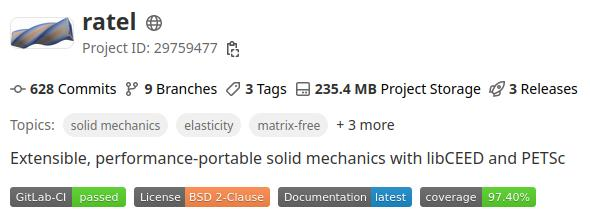
\includegraphics[height=3.0cm]{ratel-badges}

~\\

Ratel is very young - 'move fast and break things'\\

~\\

Best practices from libCEED, PETSc break fewer things\\

~\\

\end{center}
\end{frame}
 
%------------------------------------------------

\begin{frame}
\frametitle{Overview} % Table of contents slide, comment this block out to remove it
\tableofcontents % Throughout your presentation, if you choose to use \section{} and \subsection{} commands, these will automatically be printed on this slide as an overview of your presentation
\end{frame}

%------------------------------------------------
\section{CI Testing}
%------------------------------------------------

\begin{frame}
\begin{center}
\frametitle{CI for commits and MRs}

CI is as essential part of MR acceptance

~\\

\begin{itemize}

\item Automated testing for every commit and merge request

~\\

\item Testing multiple hardware and build configurations

~\\

\item Automatic static code analysis and formatting

\end{itemize}

~\\

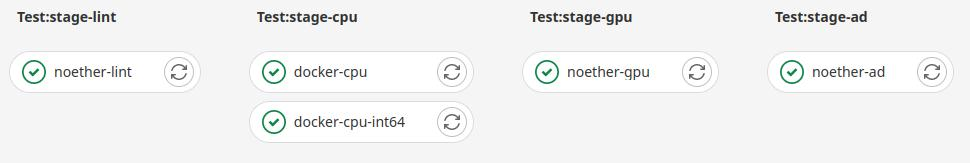
\includegraphics[height=2.0cm]{ratel-ci-tests}

\end{center}
\end{frame}

%------------------------------------------------

\begin{frame}
\begin{center}
\frametitle{Unit testing}

\begin{itemize}

\item Leverage upstream testing to lower test burden\\

~\\

\item Linear model MMS to test solver setup\\

~\\

\item Non-linear model regression tests\\

~\\

\item Untested code is broken code; tested code is less broken code\\

\end{itemize}

\end{center}
\end{frame}

%------------------------------------------------

\begin{frame}
\begin{center}
\frametitle{Code coverage}

\begin{itemize}

\item GitLab has native support for code coverage reports\\

~\\

\item Highlights vulnerable, untested code in MR diffs\\

~\\

\item Untested code is broken code; tested code is less broken code\\

\end{itemize}

~\\

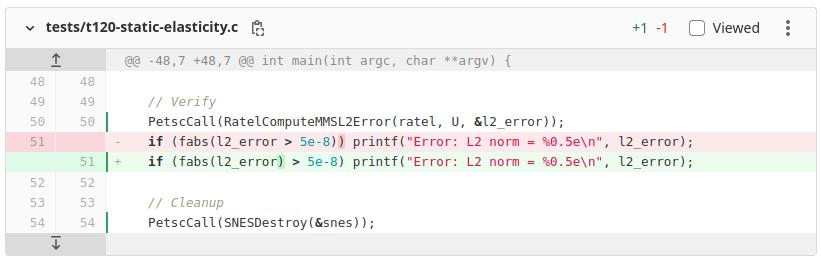
\includegraphics[height=2.5cm]{ratel-mr-coverage}

\end{center}
\end{frame}

%------------------------------------------------

\begin{frame}
\begin{center}
\frametitle{Static analysis}

\lstinline{clang-tidy} - Clang-based C++ “linter” tool\\

~\\

\begin{itemize}

\item Extensible framework for diagnosing typical errors - style violations, interface misuse, etc

\end{itemize}

~\\

{\it ClangFormat} - formatting tools built on top of LibFormat\\

~\\

\begin{itemize}

\item Standalone tool with editor integrations\\

~\\

\item Prevents format wars bikeshedding

\end{itemize}

\end{center}
\end{frame}

%------------------------------------------------
\section{CD Containers and Documentation}
%------------------------------------------------

\begin{frame}
\begin{center}
\frametitle{Automated deployment}

Automatic deployment upon commit to main\\

~\\

\begin{itemize}

\item Docker images for dev environment and latest snapshot

~\\

\item GitLab pages documentation and theory guide

\end{itemize}

~\\

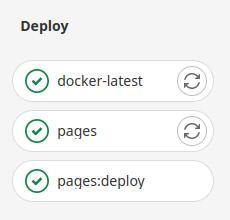
\includegraphics[height=2.5cm]{ratel-cd-docker-and-docs}

\end{center}
\end{frame}

%------------------------------------------------

\begin{frame}[fragile]
\begin{center}
\frametitle{Docker containers}

Snapshot and dev environment images\\

~\\

\begin{itemize}

\item User quick start with general CPU only image\\

~\\

\item Exact dependency commit hashes shipped with Dockerfiles\\

\end{itemize}

~\\

\begin{lstlisting}[language=bash, basicstyle=\ttfamily\scriptsize]
host$ docker run -it --rm -v $(pwd):/work registry.gitlab.com/micromorph/ratel
container$ ratel-quasistatic -options_file config.yaml
\end{lstlisting}

\end{center}
\end{frame}

%------------------------------------------------

\begin{frame}
\begin{center}
\frametitle{Documentation}

Latest documentation and theory guide\\

~\\

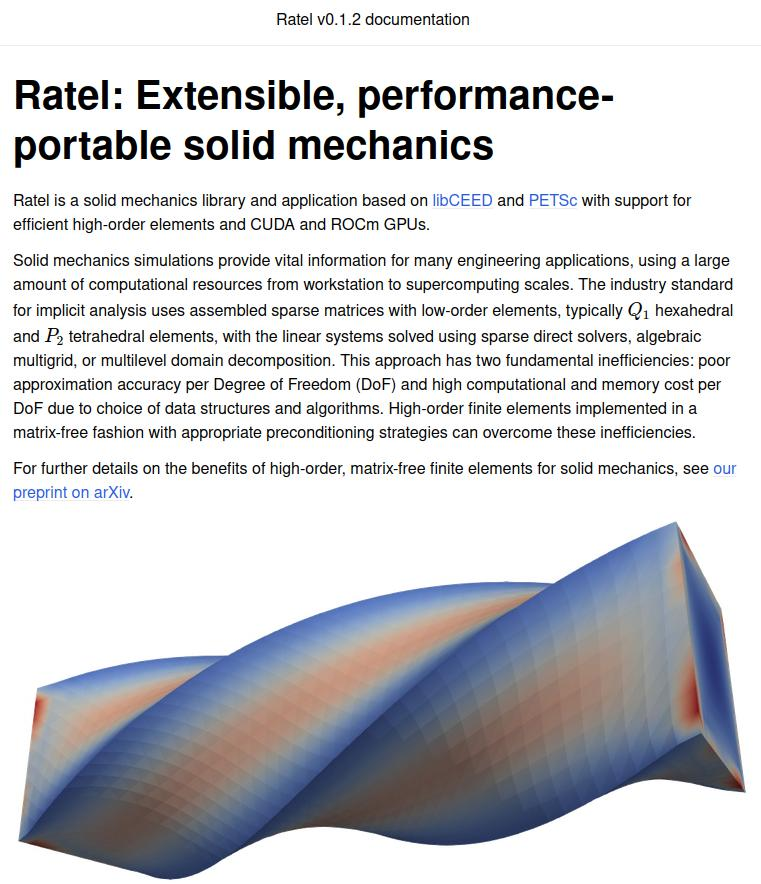
\includegraphics[height=5cm]{ratel-docs}

\end{center}
\end{frame}

%------------------------------------------------
\section{Issue Tracker}
%------------------------------------------------

\begin{frame}
\begin{center}
\frametitle{Issue tracker}

\begin{itemize}

\item Transparent development roadmap\\

\end{itemize}

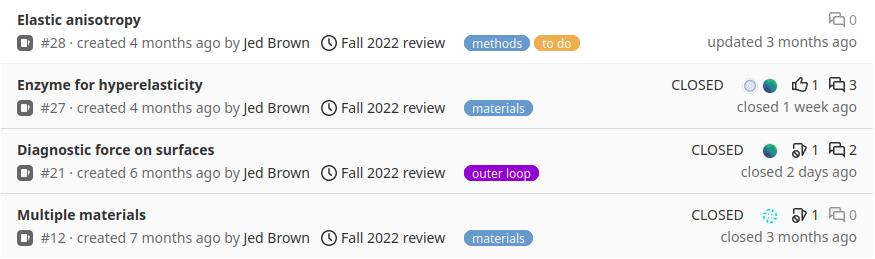
\includegraphics[height=2.5cm]{ratel-dev-roadmap}

\begin{itemize}

\item Bug tracker\\

\end{itemize}

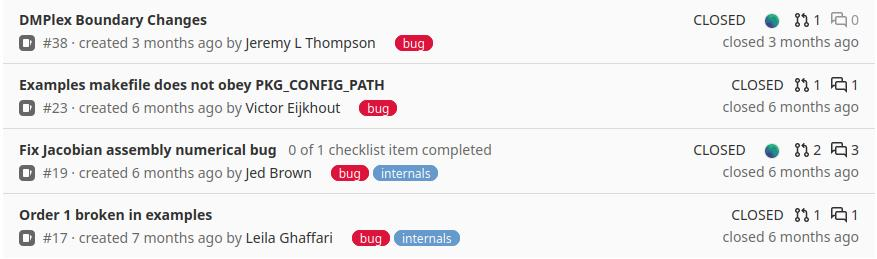
\includegraphics[height=2.5cm]{ratel-bug-tracker}

\end{center}
\end{frame}

%------------------------------------------------
\section{Community Contributions}
%------------------------------------------------

\begin{frame}
\begin{center}
\frametitle{Upstream contributions}

Upstream improvements to libCEED and PETSc

~\\

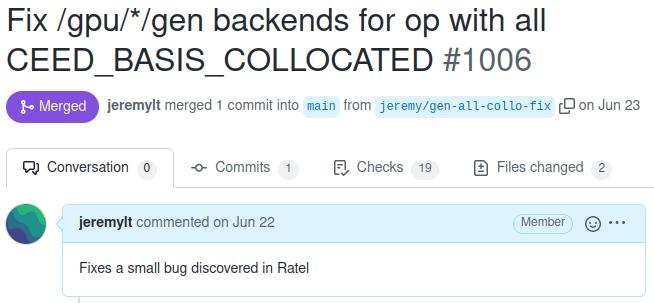
\includegraphics[height=3cm]{ratel-libceed-upstream}

~\\

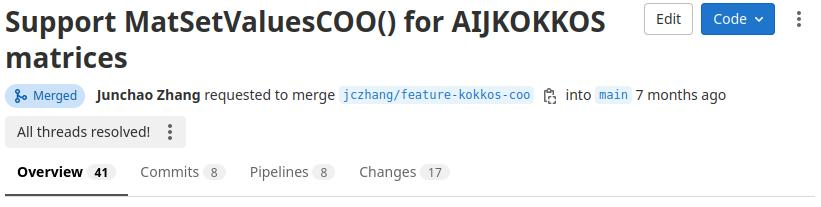
\includegraphics[height=2cm]{ratel-petsc-upstream}

\end{center}
\end{frame}
 
%------------------------------------------------

\begin{frame}
\frametitle{Questions?} % Table of contents slide, comment this block out to remove it
\tableofcontents % Throughout your presentation, if you choose to use \section{} and \subsection{} commands, these will automatically be printed on this slide as an overview of your presentation
\end{frame}

%-------------------------------------------------------------------------------

\end{document}

%-------------------------------------------------------------------------------
